% 第6章第4节：图谱与连通性（特征向量与变化尺度、零空间与连通分量、归一化谱界）。

\section{图谱与连通性}
\label{sec:graph-spectrum-connectivity}

前两节建立的$\bm L$与$\bm L_{\mathrm{sym}}$都是实对称矩阵，可以直接使用第三部分的谱定理。本节回答三个问题：特征向量表示怎样的变化模式，零特征值反映了图的什么结构，归一化后的特征值落在什么范围。所选图算子的特征值合起来称为\term{图谱}（graph spectrum）。它由算子和边权决定，不由顶点编号决定，也不是事先给定的物理频率。

\subsection{特征向量与变化尺度}
\label{sec:graph-spec-eigenvectors-scales}

由谱定理（定理~\ref{thm:ls-real-symmetric-spectral}），存在正交矩阵$\bm U=[\bm u_1,\ldots,\bm u_n]$与实对角矩阵$\bm\Lambda$，使
\begin{equation}
 \bm L=\bm U\bm\Lambda\bm U^{\top},\qquad
 \bm\Lambda=\operatorname{diag}(\lambda_1,\ldots,\lambda_n),\qquad
 \lambda_1\leq\lambda_2\leq\cdots\leq\lambda_n .
 \label{eq:graph-spec-laplacian-eigendecomposition}
\end{equation}
按本章约定，特征值从小到大编号。$\bm L$半正定，所以全部$\lambda_k\geq0$；又$\bm L\bm1=\bm0$，所以$\lambda_1=0$。

特征值有一个直接的含义。对单位特征向量$\bm u_k$，
\[
 \bm u_k^{\top}\bm L\bm u_k=\lambda_k\bm u_k^{\top}\bm u_k=\lambda_k ,
\]
即$\lambda_k$就是$\bm u_k$的沿边变化能量。由于长度已经固定为$1$，小特征值对应沿边起伏小的方向，大特征值对应相邻顶点取值差异大的方向。因此常把$\lambda_k$称为\term{图频率}（graph frequency）：把特征值看作频率，特征向量看作该频率的振荡模式，低频平缓、高频剧烈。

\begin{figure}[!htb]
  \centering
  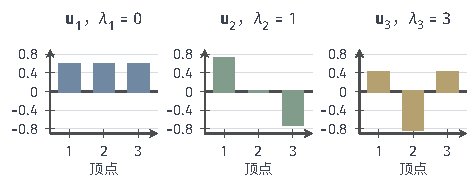
\includegraphics[width=80mm]{figures/01-basic-mathematics/04-graphs/tikz/c6-path-modes/figure.pdf}
  \caption{单位权三点路径的三个标准正交特征向量，条高为各顶点上的取值。$\bm u_1$为常量，能量$0$；$\bm u_2$两端反号、中间为零，变号一次，能量$1$；$\bm u_3$中间与两端反号，变号两次，能量$3$。}
  \label{fig:graph-spec-path-modes}
\end{figure}

单位权三点路径的拉普拉斯可以逐个核对。取
\[
 \bm u_1=\tfrac1{\sqrt3}(1,1,1)^{\top},\qquad
 \bm u_2=\tfrac1{\sqrt2}(1,0,-1)^{\top},\qquad
 \bm u_3=\tfrac1{\sqrt6}(1,-2,1)^{\top}.
\]
直接相乘得$\bm L(1,0,-1)^{\top}=(1,0,-1)^{\top}$、$\bm L(1,-2,1)^{\top}=(3,-6,3)^{\top}$，所以对应特征值为$0,1,3$。用能量逐边核对：$\bm u_2$在两条边上的差都是$\tfrac1{\sqrt2}$，能量$\tfrac12+\tfrac12=1$；$\bm u_3$在两条边上的差都是$\tfrac3{\sqrt6}$，能量$\tfrac96+\tfrac96=3$。图~\ref{fig:graph-spec-path-modes}显示，从常量到左右反向、再到中间与两端反向，变号次数增加，能量随之增大。

图频率依赖边权。把边$\{2,3\}$的权从$1$改为$4$，拉普拉斯变为
\[
 \begin{bmatrix}1&-1&0\\-1&5&-4\\0&-4&4\end{bmatrix},
\]
除零之外的两个特征值满足$\lambda^2-10\lambda+12=0$，即$5\pm\sqrt{13}\approx1.39,\,8.61$。连接关系和顶点次序都没变，谱却变了。所以不能把图频率看成只由无权连接或数组次序决定的固定量。

\paragraph{重编号下的谱}
第~\ref{sec:graph-isomorphism}节用置换矩阵$\bm P$表示顶点重编号，邻接矩阵变为$\bm P\bm A\bm P^{\top}$。度矩阵与权矩阵同步重排，所以拉普拉斯变为$\bm L'=\bm P\bm L\bm P^{\top}$。若$\bm L\bm u=\lambda\bm u$，由$\bm P^{\top}\bm P=\bm I$，
\[
 \bm L'(\bm P\bm u)=\bm P\bm L\bm P^{\top}\bm P\bm u=\bm P\bm L\bm u=\lambda\,\bm P\bm u .
\]
特征值不变，特征向量的分量随顶点一起重排。这区分了三个层次：记录顺序是任意选择的；特征向量在某个记录顺序下的坐标随顺序改变；图谱本身则不依赖记录顺序，是同构图共有的量。

\subsection{零空间与连通分量}
\label{sec:graph-spec-null-space-components}

第~\ref{sec:graph-spec-dirichlet-energy}小节得到了逐边条件：能量为零当且仅当每条正权边两端相等。把这个条件沿路径传递，就能确定全部零特征向量。下面的$\bm1_C$表示顶点集$C$的指示向量，在$C$上取$1$、其余为$0$；连通分量的概念见第~\ref{sec:graph-connectivity-separation}节。

\begin{theorem}[零空间与正权支撑分量]
\label{thm:graph-spec-null-space}
设$\mathcal G$为有限无向图，边权非负对称，正权支撑图$(V,E_+)$的连通分量为$C_1,\ldots,C_c$，则
\[
 \ker\bm L=\operatorname{span}\{\bm1_{C_1},\ldots,\bm1_{C_c}\},
\]
且$\bm L$的零特征值的重数等于$c$。
\end{theorem}

\begin{proof}
第一步，零空间由能量刻画。若$\bm L\bm f=\bm0$，则$\bm f^{\top}\bm L\bm f=\bm f^{\top}\bm0=0$。反过来，把$\bm f=\sum_kc_k\bm u_k$代入，$\bm f^{\top}\bm L\bm f=\sum_k\lambda_kc_k^2$，各项非负，和为零迫使$\lambda_k>0$时$c_k=0$，于是$\bm L\bm f=\sum_k\lambda_kc_k\bm u_k=\bm0$。所以$\bm L\bm f=\bm0$当且仅当$\bm f^{\top}\bm L\bm f=0$，又当且仅当每条正权边两端相等。

第二步，相等关系沿路径传递。若$i$与$j$在同一分量$C$中，则存在一条只经过正权边的路径$i=v_0,v_1,\ldots,v_\ell=j$，逐边得$f_{v_0}=f_{v_1}=\cdots=f_{v_\ell}$。所以零能量的函数在每个分量上取常数。反之，正权边的两个端点总在同一分量中，在各分量上分别取常数的函数，在每条正权边上的差都为零。于是$\ker\bm L$恰为“在每个分量上取常数”的函数全体，每个这样的函数都可写成$\sum_ta_t\bm1_{C_t}$。

第三步，数维数。各分量互不相交，指示向量的支撑互不重叠，两两正交，因而线性无关，$\dim\ker\bm L=c$。在谱分解~\eqref{eq:graph-spec-laplacian-eigendecomposition}中，$\ker\bm L$由$\lambda_k=0$的那些$\bm u_k$张成，所以零特征值恰好出现$c$次。
\end{proof}

这一结论特别给出：$\lambda_2>0$当且仅当正权支撑图连通。图~\ref{fig:graph-spec-component-null-modes}中的图有三个正权支撑分量：路径$\{1,2,3\}$、边$\{4,5\}$和孤点$6$，所以零特征值的重数为$3$（直接计算可得$\bm L$的谱为$0,0,0,1,2,3$）。连接$3$与$4$的零权边结构上存在，但它的能量项恒为零，不迫使两端相等，所以不能把两个分量合并：$\bm1_{C_1}$与$\bm1_{C_2}$可以分别取不同的常数。

\begin{figure}[!htb]
  \centering
  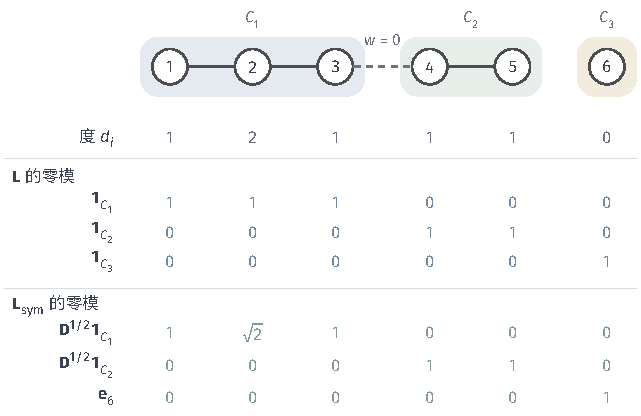
\includegraphics[width=108mm]{figures/01-basic-mathematics/04-graphs/tikz/c6-component-null-modes/figure.pdf}
  \caption{正权支撑分量与零特征向量。实线为单位权边，虚线$\{3,4\}$为零权结构边，顶点$6$为支撑孤点；三块底色标出分量$C_1,C_2,C_3$。上半部分为$\bm L$零空间的一组基，即各分量的指示向量；下半部分为$\bm L_{\mathrm{sym}}$零空间的一组基：正度分量上是度缩放的指示向量$\bm D^{1/2}\bm1_C$，孤点处是坐标方向$\bm e_6$。两组基的个数相同，向量不同。}
  \label{fig:graph-spec-component-null-modes}
\end{figure}

\paragraph{归一化算子的零空间}
同样的论证可以搬到$\bm L_{\mathrm{sym}}$。在正度顶点上，由式~\eqref{eq:graph-spec-normalized-energy}，能量为零当且仅当每条正权边上$f_i/\sqrt{d_i}=f_j/\sqrt{d_j}$，即$\bm D^{-1/2}\bm f$在每个分量上取常数。所以每个含正权边的分量$C$贡献零特征向量$\bm D^{1/2}\bm1_C$。支撑孤点$v$的行与列全为零，坐标方向$\bm e_v$也是零特征向量。合起来，$\bm L_{\mathrm{sym}}$的零特征值重数仍等于正权支撑分量数（孤点自成一个分量），但基向量换成了度缩放的版本。图~\ref{fig:graph-spec-component-null-modes}的下半部分列出了它们，例如$\bm D^{1/2}\bm1_{C_1}=(1,\sqrt2,1,0,0,0)^{\top}$。

普通常量与度缩放常量不能互换。图~\ref{fig:graph-spec-three-laplacians}(b)已经显示$\bm L_{\mathrm{sym}}\bm1\neq\bm0$；只有在一个分量内各点度相同时，二者才成比例。至于$\bm L_{\mathrm{rw}}$，它在正度行上等于$\bm D^{-1}\bm L$，在孤点行上为零，所以$\bm L_{\mathrm{rw}}\bm g=\bm0$当且仅当$\bm L\bm g=\bm0$，零空间仍由普通的分量指示向量张成。

\subsection{归一化谱界}
\label{sec:graph-spec-normalized-bound}

组合拉普拉斯的特征值随边权整体放缩：所有边权乘以$c>0$，$\bm L$乘以$c$，谱也乘以$c$。$\bm L_{\mathrm{sym}}$则不受这种放缩影响，因为$\bm D^{-1/2}$同时乘以$c^{-1/2}$，两侧抵消。下面证明它的特征值总在一个固定区间内。

\begin{theorem}[归一化谱界]
\label{thm:graph-spec-normalized-bound}
对有限无向非负权图，按本节约定定义的$\bm L_{\mathrm{sym}}$满足$0\leq\bm f^{\top}\bm L_{\mathrm{sym}}\bm f\leq2\lVert\bm f\rVert_2^2$，因此它的全部特征值落在$[0,2]$中。
\end{theorem}

\begin{proof}
下界即式~\eqref{eq:graph-spec-normalized-energy}的非负性。对上界，对任意实数$a,b$有$(a-b)^2\leq2(a^2+b^2)$，因为两边之差为$(a+b)^2\geq0$。令$a_i=f_i/\sqrt{d_i}$（$i\in V_+$），逐边使用这一不等式：
\[
 \begin{aligned}
 \sum_{\{i,j\}\in E_+}w_{i,j}(a_i-a_j)^2
 &\leq2\sum_{\{i,j\}\in E_+}w_{i,j}\bigl(a_i^2+a_j^2\bigr)
 =2\sum_{i\in V_+}a_i^2\sum_jw_{i,j}\\
 &=2\sum_{i\in V_+}\frac{f_i^2}{d_i}\,d_i\leq2\lVert\bm f\rVert_2^2 .
 \end{aligned}
\]
中间的等号把每条边上的两项分别归到两个端点，每个顶点$i$收集到的权之和恰为$d_i$；最后一步只是丢掉了支撑孤点上的非负项$f_v^2$。设$\bm x_k$是$\bm L_{\mathrm{sym}}$的单位特征向量，特征值为$\mu_k$，取$\bm f=\bm x_k$即得$0\leq\mu_k=\bm x_k^{\top}\bm L_{\mathrm{sym}}\bm x_k\leq2$；也可以由Rayleigh--Ritz定理（定理~\ref{thm:matrix-analysis-rayleigh-ritz}）读出。
\end{proof}

上界可以取到。单位权三点路径的$\bm L_{\mathrm{sym}}$特征值为$0,1,2$，取到$2$的特征向量是$(1,-\sqrt2,1)^{\top}$，换回原坐标$\bm D^{-1/2}\bm f=(1,-1,1)^{\top}$，相邻顶点正负交替，每条边都达到证明中不等式的等号$a_i=-a_j$。组合拉普拉斯没有同样的统一上界：这条路径的$\bm L$已有特征值$3>2$。同样的论证只给出$\bm f^{\top}\bm L\bm f\leq2\sum_id_if_i^2\leq2d_{\max}\lVert\bm f\rVert_2^2$，上界随最大度和边权的尺度变化。

谱界告诉我们特征值可能出现在哪个区间。第~\ref{sec:graph-filtering}节设计滤波响应、用多项式逼近响应时，只需在这个区间上考虑。谱界本身不是任何迭代算法的收敛保证，那需要另行分析。
